%!TEX root = ../thesis.tex
%*******************************************************************************
%*********************************** First Chapter *****************************
%*******************************************************************************

\chapter{Aplicaciones de la minería de datos en ingeniería de proteínas}  %Title of the First Chapter

\ifpdf
    \graphicspath{{Chapter1/Figs/Raster/}{Chapter1/Figs/PDF/}{Chapter1/Figs/}}
\else
    \graphicspath{{Chapter1/Figs/Vector/}{Chapter1/Figs/}}
\fi

La ingeniería de proteínas, es una de las ramas más relevantes y de mayor impacto en el campo de la biotecnología. Su objetivo principal, se basa en el diseño de mutaciones, enfocadas en adicionar características específicas o mejorar sus propiedades fisicoquímicas, ya sea para someterlas a distintos tipos de ambientes, adecuarla a interactuar con diferentes elementos, presentar una mayor estabilidad, etc. \cite{lutz2009protein}.

Los diseños de mutaciones se resumen en dos técnicas principales: El diseño racional \cite{carpenter1997rational} y la evolución dirigida \cite{arnold1998design}, ambas técnicas experimentales, que cumplen con el mismo objetivo, relacionado a alterar las propiedades de la proteína para provocar una mejora con respecto a la estructura inicial.

A pesar de que ambas técnicas son utilizadas día a día, en diferentes investigaciones, éstas presentan limitantes importantes, en particular, relacionadas con el espacio de búsqueda posible a explorar, el tiempo que conlleva realizar diferentes pruebas y el costo económico y de recursos humanos que implica evaluar diferentes mutaciones \cite{Reetz2008}. 

Diferentes métodos computacionales han sido desarrollados, enfocados principalmente en el estudio de proteínas y el apoyo al diseño de mutaciones. Estas herramientas, se centran en el análisis de la estructura y la estabilidad termodinámica de sustituciones, adiciones o eliminaciones de residuos \cite{Schymkowitz2005, Khan2010, Pandurangan2017, Olivera-Nappa2011}. Sin embargo, debido a cómo estos funcionan, en ocasiones, el costo computacional es muy elevado, ya que escala linealmente con respecto a la cantidad de pruebas a realizar. 

Por otro lado, métodos basados en técnicas de minería de datos y aprendizaje de máquinas, se presentan como una alternativa potente y de costo computacional reducido, siendo capaces de generar resultados a partir de conocimiento existente, ya sea, para entrenar modelos que permitan evaluar mutaciones desde puntos de vista de estabilidad, identificación de residuos relevantes en propiedades fisicoquímicas, evaluar propensiones a cambios, etc. \cite{Capriotti2005, softwareVHL, article}. 

No obstante, dado el gran volumen de datos existente en la actualidad ¿cómo es posible reconocer qué dato es relevante y cuál no?, ¿cómo puedo representar la información existente?, ¿cómo puedo complementar las diversas técnicas experimentales desarrolladas con el enfoque de la minería de datos?, etc., son interrogantes que nacen a partir del uso de técnicas computacionales y el apoyo a las metodologías experimentales.

Dado lo anterior, durante el presente capítulo, se expone el concepto de ingeniería de proteínas y cuáles son las principales técnicas experimentales involucradas en el diseño de mutaciones. Además se introduce el concepto de Minería de datos y se exponen diversas metodologías computacionales que han sido desarrolladas, enfocadas en este campo de investigación. Por último, se presentan diferentes problemas que dan el punto de partida a cada una de las propuestas metodológicas de esta tesis doctoral y que denotan la evidente necesidad de ser desarrolladas o que exponen cambios en los puntos de vista actuales asociados al desarrollo de modelos y las convierten en un aporte significativo a los estudios actuales de mutaciones y el diseño de proteínas. 

\section{Ingeniería de proteínas \label{cap1:sec1}}

Por definición, la ingeniería de proteínas, es un campo de investigación centrado en el diseño y creación de proteínas útiles o con propiedades fisicoquímicas relevantes, con un enfoque relevante en la comprensión del plegamiento de proteínas.

Actualmente, la ingeniería de proteínas, cuenta con dos estrategias principales para la construcción de mutaciones. Siendo éstas la evolución dirigida y el diseño racional. Sin embargo, a pesar de su existencia, normalmente no son excluyentes, por lo que es común utilizar ambas metodologías. No obstante, un estudio completo de residuos y una evaluación detallada de las sustituciones es una limitante importante para estas dos técnicas, debido tanto a recursos económicos como humanos.

La evolución dirigida imita el proceso de selección natural, permitiendo direccionar la evolución hacia objetivos definidos, reflejados en cuanto a funciones o propiedades fisicoquímicas deseables. Una representación del proceso, se observa en la Figura \ref{ed}. 


\begin{figure}[!h]
	
	\centering
	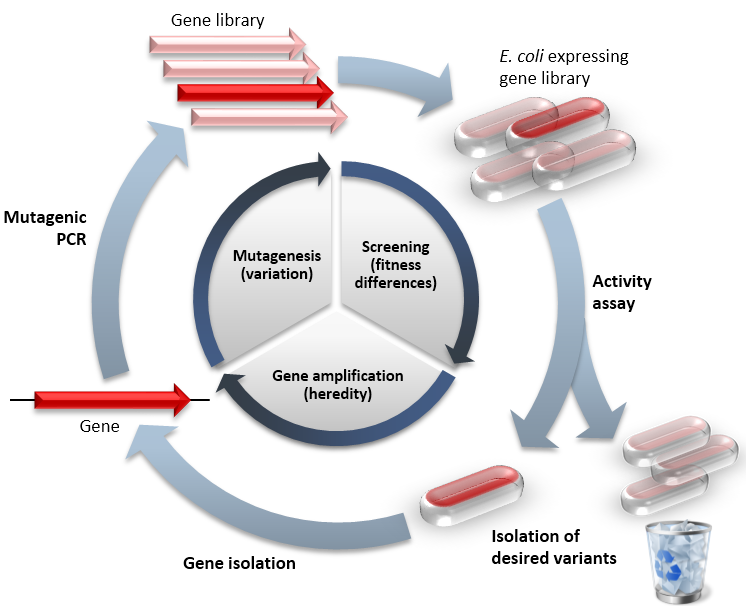
\includegraphics[scale=.6]{DEcycle.png}
	\caption{Esquema representativo de los pasos que contempla la evolución dirigida}
	\label{ed}
\end{figure}

El proceso, de manera general, consiste en someter un gen de interés a rondas iterativas de mutagénesis, con el fin de crear una biblioteca de variantes. A partir de dicho conjunto de elementos, se seleccionan las variantes con la función deseada. Finalmente, se aíslan y se amplifican para forman una plantilla para la siguiente iteración. Así el proceso sigue iterando y estadísticamente, se seleccionan las más favorables y aquellas que tendieron a la evolución debido a la supervivencia en el proceso.

Con respecto al diseño racional de proteínas. Ésta, es una técnica ampliamente utilizada y al igual que la evolución dirigida, presenta el objetivo general de generar variantes con alguna función de interés o características particulares. No obstante, presenta una diferencia relevante, la cual se centra en la información que debe existir sobre la estructura, mecanismos, plegamiento o secuencia lineal de la proteína de interés.

\section{Métodos computacionales aplicados en ingeniería de proteínas}

Diferentes métodos computacionales han sido desarrollados para distintos análisis, con el fin de poder 

\section{Minería de datos}


Minería de datos es el proceso de descubrimiento de patrones en set de datos, involucrando métodos asociados a Machine Learning \cite{michie1994machine}, Estadísticas y sistemas de bases de datos. \cite{hand2006data}. La minería de datos es un subcampo interdisciplinario de la informática, el cual tiene por objetivo general extraer información (a través de métodos inteligentes) de un conjunto de datos y transformar la información en una estructura comprensible para su uso posterior. \cite{fayyad1996knowledge, dunham2006data}. 

La minería de datos es el paso de análisis del proceso de \textit{descubrimiento de conocimiento en bases de datos}, o KDD. \cite{fayyad1996kdd}. Además, del análisis en bruto de los datos, también incluye aspectos de manipulación de bases de datos y pre procesamiento de estos, evaluaciones de modelo e inferencia, métricas de interés, consideraciones de complejidad, post procesamiento de estructuras descubiertas, visualización y actualización de la información \cite{berry2004data}.

En la Figura \ref{intro1}, se exponen las principales ramas que componen la minería de datos y los diferentes procesos que se asocian a dichas ramas.

\begin{figure}[!h]
	
	\centering
	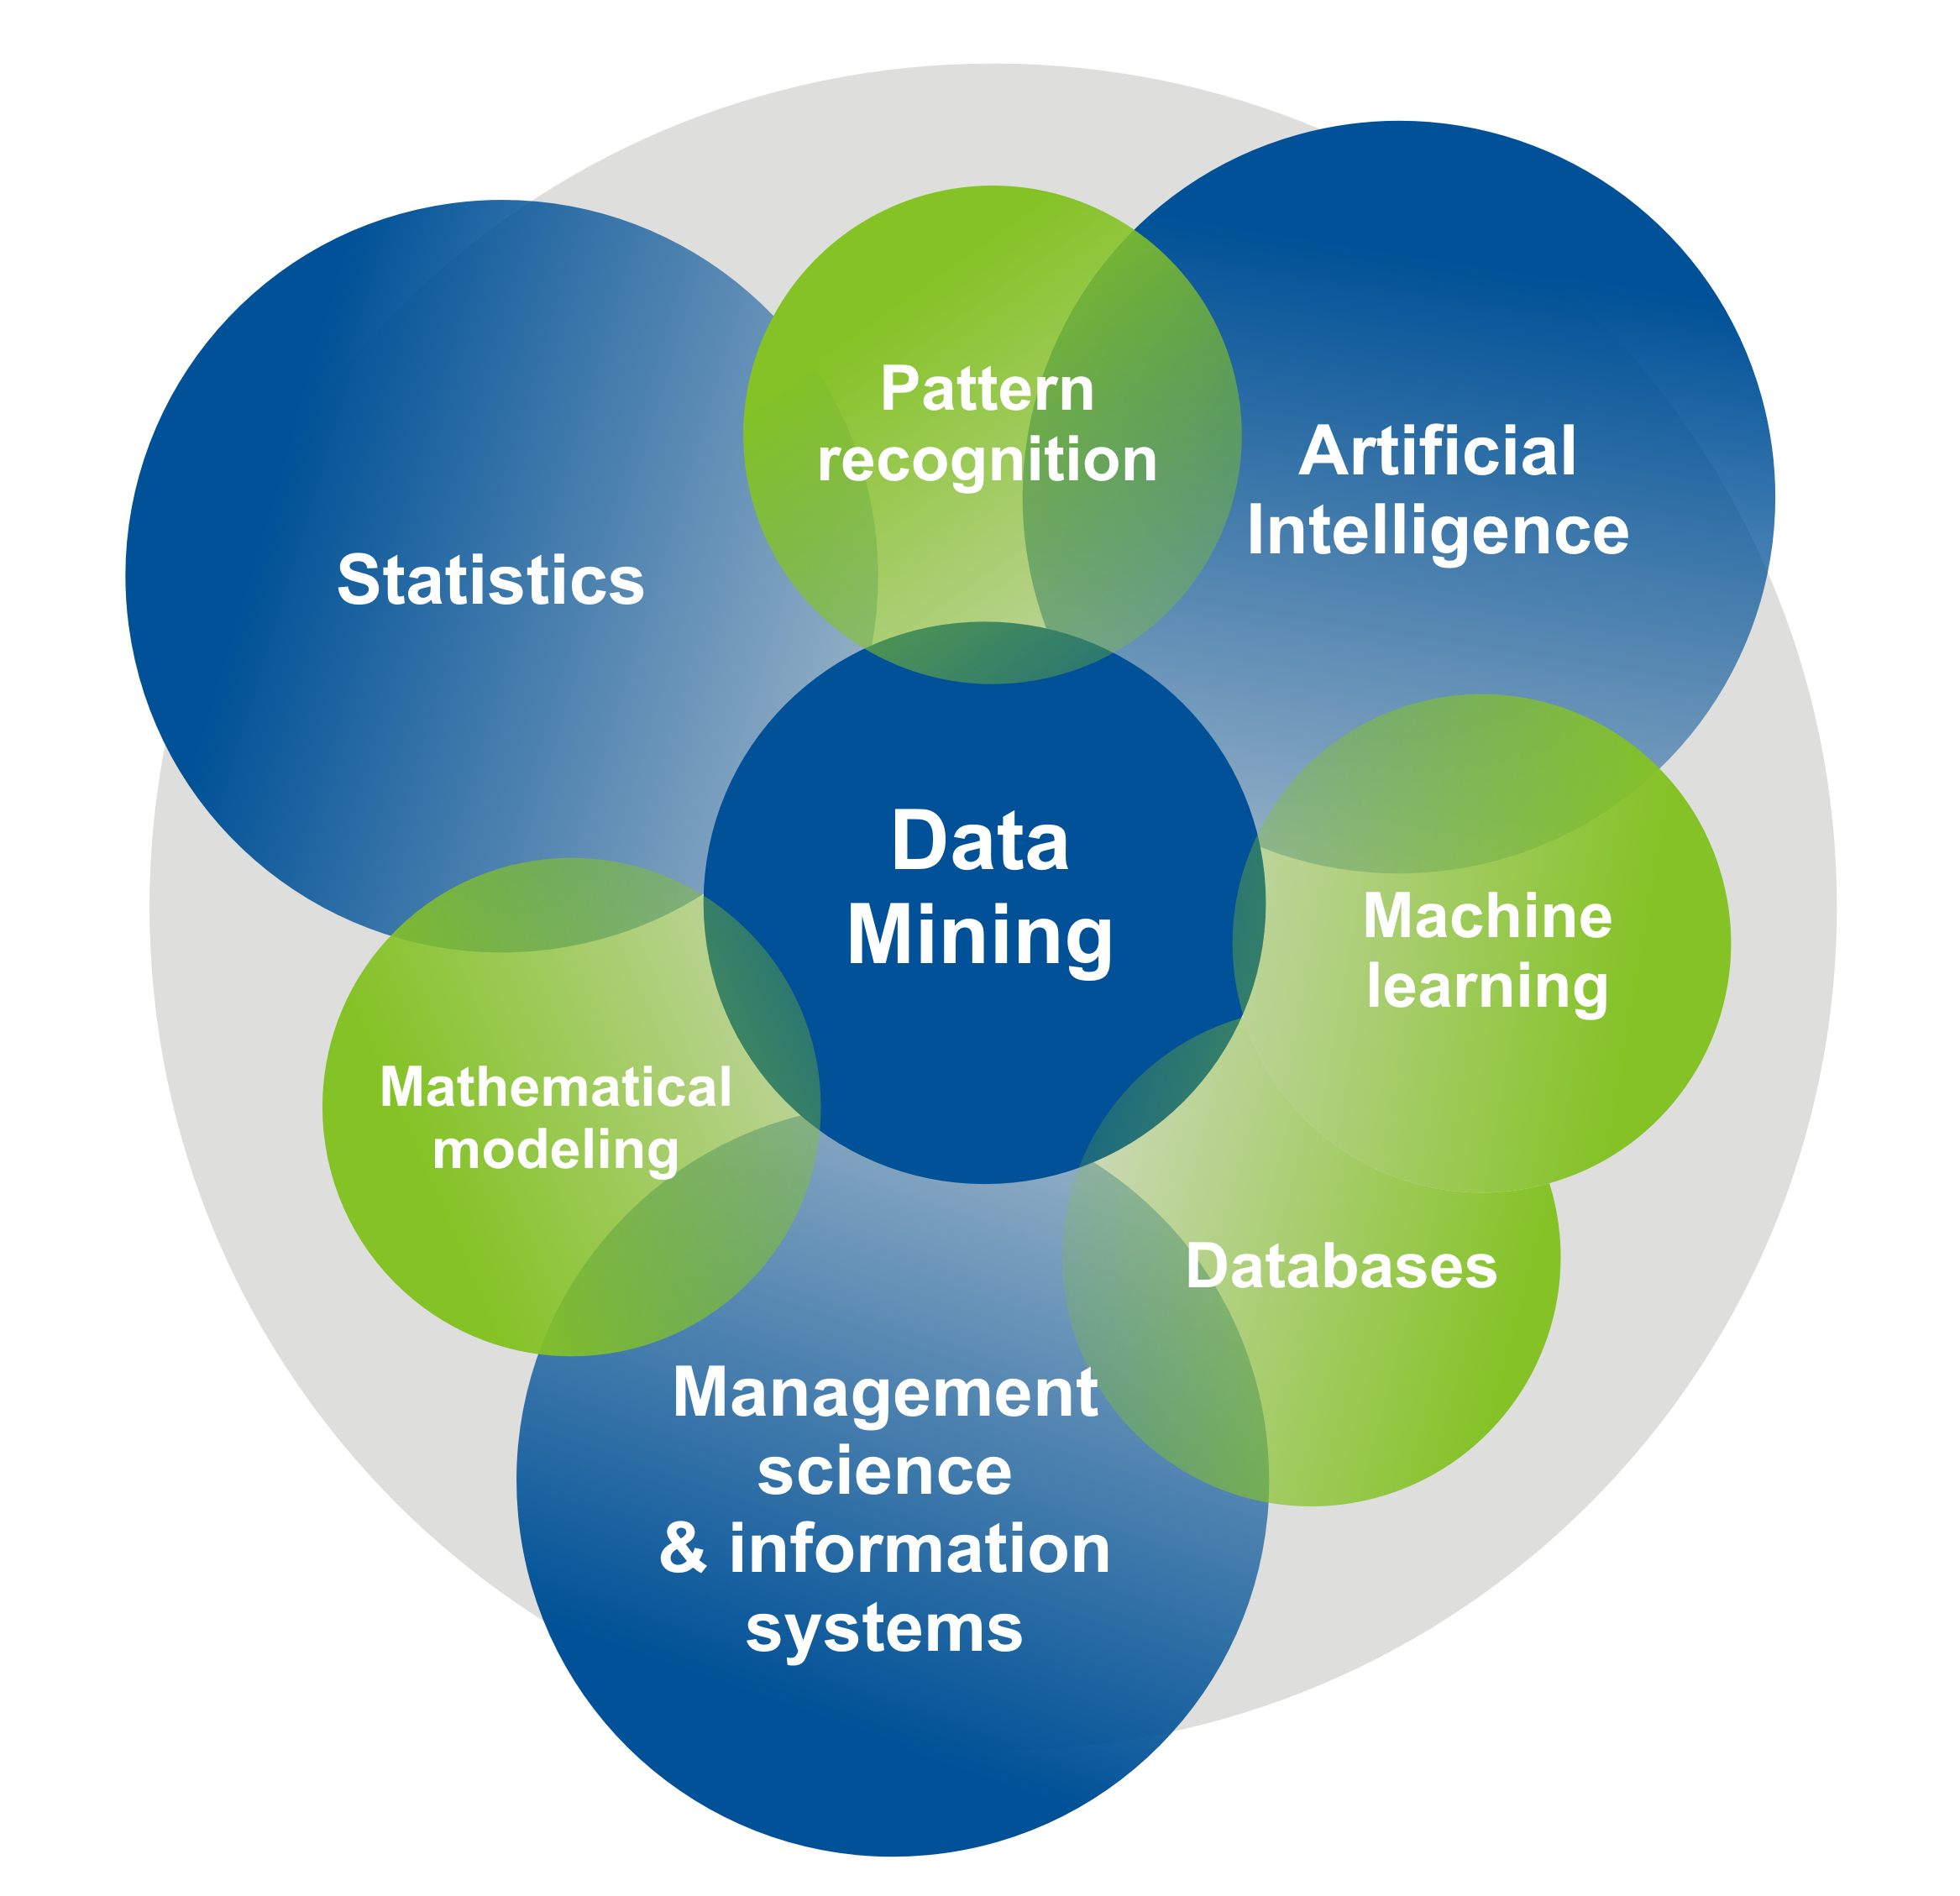
\includegraphics[scale=.4]{dataMining.jpg}
	\caption{Componentes principales de la minería de datos}
	\label{intro1}
\end{figure}

Son tres las principales áreas que abarca la minería de datos: Estadística, Inteligencia Artificial y Manipulación de sistemas de información. Por otro lado, son distintos procesos los que interactúan entre estas ramas, tales como: Modelamiento Matemático, reconocimiento de patrones, Sistemas de almacenamiento persistente y machine learning \cite{hand2006data}.

Cada área en particular, tiene un objetivo general y diversos objetivos específicos. Sin embargo, estas áreas interactúan entre sí, con el fin de poder extraer patrones de información que generen conocimientos a partir de la data de procesada \cite{berry2004data}.

La minería de datos se utiliza en diferentes campos, tales como: genética y genómica \cite{Lee2008, Rebhan1998}, ingeniería de proteínas \cite{han2009research, 4548625, li2008fast}, comercio y negocios \cite{hofmann2013rapidminer}, sistemas de tránsito \cite{Ma2013}, optimizaciones en procesos industriales \cite{Chien2008, 8051033, 983448}, reconocimiento de patrones \cite{jain1988algorithms, fayyad1996data}, rasgos cuantificables en enfermedades \cite{Yoo2012, obenshain2004, LDuan} y más recientemente en áreas de dinámicas moleculares \cite{Chen2017, Yang:2005:GFM:1081870.1081962} y parámetros para la generación de pipe lines automatizados de simulaciones cuánticas en sistemas químicos \cite{MAO2004787, PhysRevLett.91.135503, Ramakrishnan2015}.


\section{Principales problemáticas en la ingeniería de datos}

Diferentes son las problemáticas que pueden existir en el campo de la ingeniería de proteínas, ya sea, desde la generación de herramientas computacionales para estudiar mutaciones y su efecto de manera masiva, hasta diseño de mutaciones basados en secuencias lineales de proteínas. A continuación se presentan diferentes problemáticas existentes en el área, algunas de las cuales son motivos de estudio y desafíos a cumplir durante el presente trabajo de título.

\subsection{Diferentes respuestas, una misma solución}

El desarrollo de modelos de clasificación y/o regresión, es uno de los temas más recurrentes en el campo de la minería de datos y el aprendizaje de máquinas. Sin embargo, el hecho de asociar mutaciones a una respuesta, conlleva al problema de cómo caracterizarla, con el fin de alimentar a los algoritmos para ser entrenados. 

A raíz de esto, cuáles son los mejores descriptores para una mutación?, desde qué puntos de vista se puede hacer una caracterización? y cuáles son más relevantes?, son interrogantes que se presentan a la hora de abordar su representación, siendo problemas que han sido tratados desde un largo tiempo, sin lograr generar un consenso o una forma general de diseñar al representación. 

En un gran número de trabajos, en los cuales se ha evaluado la estabilidad de proteínas en torno a la mutación, se han utilizado descriptores termodinámicos y de ambiente para poder representar el elemento. A pesar de que los desempeños de los estimadores han sido aceptables y relativamente altos. Esta caracterización podrá ser utilizada para mutaciones asociadas a riesgo clínico? Existirá una correlación entre la respuesta y las variables de interés? Cómo afecta al desempeño del modelo la existencia de diferentes ejemplos asociados a distintas proteínas en un único conjunto de datos?, etc., son interrogantes que nacen a la hora de plantearse la situación.

Dado a lo anterior, y con el objetivo de generar un aporte significativo al desarrollo de estimadores basados en aprendizaje de máquinas, se ha propuesto adicionar el concepto de filogenia a la descripción de mutaciones y disgregar los conjuntos de elementos para ser tratados por proteínas independientes, esto con el fin de generar modelos de clasificación y/o regresión proteína-específicos, los cuales puedan ser aplicados a diferentes respuestas de interés ya sea: efectos en mutaciones, estabilidad, actividad, productividad, etc., siendo éste, el tema central a abordar en el capítulo \ref{cap2}.
 
\subsection{Codificaciones, cuáles es la mejor alternativa?}

A menudo, el uso de secuencias lineales de proteínas se relaciona a la identificación de patrones o evaluación de variantes para una misma proteína. Actuales herramientas bioinformáticas permiten el uso de la secuencia de manera directa y por medio de alineamientos de secuencias o modelamiento a través del uso de Cadenas de Markov permiten el reconocimiento de patrones o la evaluación de mutaciones. No obstante, para la aplicación de métodos basados en minería de datos, ya sea la identificación de clusters o el entrenamiento de modelos, se requiere codificar la secuencia.

Existen diferentes codificaciones posibles, ya sea, para representar la secuencia o para la caracterización de mutaciones. A pesar de ello, no existe un consenso asociado a qué técnica utilizar. Cada una presenta sus pros y contra. No obstante, la cantidad de información involucrada varía entre ellas. Sin embargo, a mayor información, incrementa el número de dimensiones a tratar, aumentando la complejidad del problema. Esto implica, utilizar técnicas de reducción de dimensionalidad para seleccionar las dimensiones con mayor variabilidad en el conjunto de datos.

Una de las codificaciones más novedosas ha sido el uso de las propiedades fisicoquímicas de los residuos y su digitalización mediante transformadas de Fourier. Esto ha permitido la identificación de residuos claves en la propiedad en estudio y soluciona el problema del efecto del ambiente de los elementos participantes.

En vista de las necesidades de desarrollo de modelos de clasificación/regresión o la identificación de residuos claves y la generación de sistemas de clustering para secuencias lineales de proteína, con el fin de apoyar al diseño de mutaciones, análisis de variantes e inclusive caracterización de secuencias, sin tener conocimiento sobre su estructura. Se propone el uso de transformadas de Fourier como método de digitalización de propiedades fisicoquímicas para el desarrollo de conjuntos de datos que permitan ser entrenados para el desarrollo de estimadores o identificar patrones, siendo el tema central a abordar en el capítulo \ref{cap3}.

\subsection{Diseñar mutaciones, un arte poco apreciado}

Diseñar mutaciones de manera eficiente, con una identificación adecuada de la propiedad en estudio o funcionalidad a adicionar, sin incurrir en grandes costos económicos y de recursos, es uno de los \textit{Santos griales} de la ingeniería de proteínas. Como se nombró previamente, son dos enfoques los que utilizan actualmente: Evolución dirigida y diseño racional de proteínas.

Ambas técnicas tienen sus ventajas y desventajas. No obstante, poseen en común una demanda en tiempo elevada y se requiere de conocimientos elevados sobre la estructura para poder diseñar las mutaciones, al menos, para el caso de diseño racional. Enfoques computacionales han sido propuestos, con el fin de minimizar los costos económicos, contemplando evaluaciones energéticas asociadas a los residuos y cómo estos afectan a la estabilidad. No obstante, no pueden ser utilizados en secuencias lineales. Además, dejan del lado el concepto filogenético en el estudio, resultado un gap entre ambos puntos de vista. Por otro lado, métodos basados en la minería de datos, sólo se han centrado en identificación de residuos o el entrenamiento de modelos para predecir estabilidad.

A partir de lo anterior, y con el fin de generar un aporte significativo en el área de diseño, se ha considerado esta problemática como un foco central y culminante para el desarrollo de este trabajo de título, proponiendo así, la implementación de una herramienta computacional, basada en técnicas de minería de datos y aprendizaje de máquinas, que permita proponer mutaciones a un conjunto de variantes con respuesta conocida. Generando la codificación de la secuencia por medio del uso de propiedades fisicoquímicas y su respectiva digitalización a través de transformadas de Fourier, seleccionando las propiedades más relevantes por medio de la aplicación de técnicas de reducción de dimensionalidad, para así, entrenar modelos de clasificación o regresión y posterior a ello, proponer mutaciones enfocadas en un filtro, aplicando herramientas de análisis de estabilidad y propensión. Toda esta problemática, el planteamiento de la metodología y qué se utilizará para llevar a cabo, se abordará en el capítulo \ref{cap4}.


\subsection{Los descartados tienen algo más que decir}

En la técnica de evolución dirigida, la selección de residuos o variantes, se basa en si presentan la característica deseable o no, o si aumenta la propiedad. Si el residuo no provoca el efecto deseado, éste es descartado, ya que no cumple con el criterio de selección.

Sin embargo, es posible pensar que, combinaciones lineales de residuos pueden provocar una sinergia en alguna propiedad, generando el resultado deseado. No obstante, el estudio de dichas combinaciones, o mejor dicho, las correlaciones asociativas existentes entre mutaciones no son consideradas, ya que, sólo se seleccionan aquellos que cumplen con dicho criterio. Pero, ¿qué pasa con aquellos residuos que son descartados y que al ser mutados al mismo tiempo con otro elemento provocan el efecto deseado, e inclusive, con mejores resultados que los brindados por los seleccionados?, ¿Existe información asociada a conjuntos de mutaciones que provoquen este efecto?, ¿Será posible idear una metodología \textit{in-silico} que permita comprender este tipo correlaciones y justificar los resultados esperados?.

Como se puede comprender, este fenómeno no ha sido explotado desde el punto de vista de minería de datos, debido principalmente, a que no existen reportes de conjuntos de datos con dichas características y esto es debido a que no ha sido un foco de estudio central. Sin embargo, se cree que es una necesidad inminente, la comprensión de estos mecanismos, ya que, aumenta el espacio de búsqueda y posterior diseño de mutaciones, en un gran número de dimensiones. Además, si bien, resultados de este estilo no han sido reportados, si, a partir de experiencias de diferentes grupos con enfoque en diseño de mutaciones y evolución dirigida, han observado que residuos no seleccionables por si solos, en combinación con otro elemento, permiten obtener la característica deseable.

A pesar de que esta problemática, no se considera dentro de los temas de estudio en sí, se plantea la discusión y se propone como un problema a ser tratado en el corto plazo, debido a las grandes implicatorias que esto puede conllevar y a las expectativas que se pueden generar al respecto, siendo de utilidad a la hora de proponer nuevas mutaciones y generar un aporte significativo en el área de ingeniería de proteínas.
 
